\subsection{Funktionsweise}
Wie bereits in Kapitel \ref{lsg:def:anpr} angeführt, besteht die Kennzeichenerkennung aus 3 Schritten. Bevor diese jedoch durchlaufen werden können, müssen zuerst alle notwendigen Bibliotheken installiert und importiert werden. Diese können mittels \verb|pip3 install <name>|, oder aber auch mit \verb|sudo apt-get install <name>| installiert werden. \\
Nachdem alle Bibliotheken und das Modul zur Überprüfung des Kennzeichens importiert wurden, beginnt mit \verb|cap = cv2.VideoCapture(0)| das Aufzeichnen des Bildes. Dieses wird durch eine Schleife ausgeführt, bis das Programm beendet wird. Falls die Kamera nicht aufgenommen werden kann, wird eine Fehlermeldung ausgegeben.
\subsubsection{Graustufenbild}
Nachdem das Bild angezeigt wurde, wird der erste Filter angewendet. Dabei handelt es sich um einen Filter, welcher das Bild in ein Graustufenbild umwandelt. Dieser wird  mit der Methode \verb|cv2.cvtColor(img, cv2.COLOR_BGR2GRAY)| aufgerufen.
\begin{figure}[H]
\centering
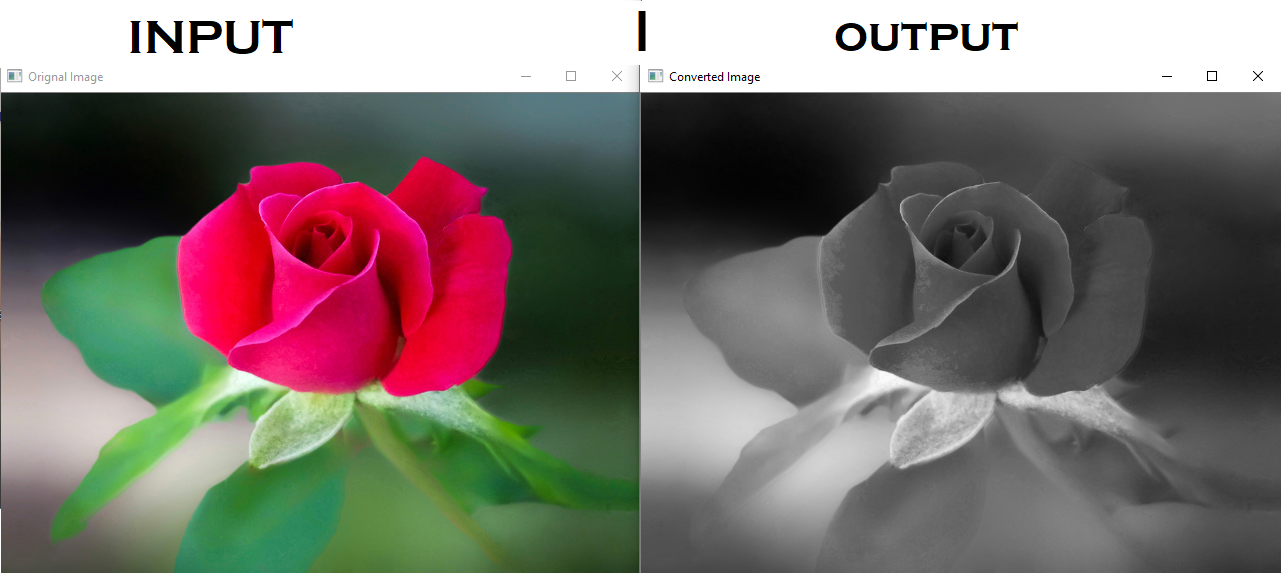
\includegraphics[width=0.8\textwidth]{pics/Color2Gray.PNG}
\caption{Aufgenommenes Bild vs. Graustufenbild}
\cite{grayscaleImage}
\label{fig:anpr_1}
\end{figure}

\subsubsection{Filter}
Als zweiter Filter fungiert ein \verb|cv2.bilateralFilter|. Die wichtigste Eigenschaft der bilateralen Filterung ist, dass sie keine Mittelwertbildung über die Kanten vornimmt. Deshalb wird sie auch als kantenerhaltender Filter bezeichnet. Bevor  die mathematischen Grundlagen des Bilateralfilters erklärt werden, ist es jedoch sinnvoll, kurz auf die Gaußsche Filterung einzugehen, da diese dem bilateralen Filter ähnlich ist.
Die Gaußsche Filterung ist ein gewichteter Durchschnitt der Intensität der benachbarten Positionen, wobei die Gewichtung mit dem räumlichen Abstand zur mittleren Position abnimmt.

Mathematisch gesehen ist ein mit Gaußscher Unschärfe gefiltertes Bild gegeben durch:
\begin{figure}[H]
    \centering
    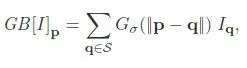
\includegraphics[width=0.5\textwidth]{pics/GBFilteredPic.jpeg}
    \caption{Ein mit Gaußscher Unschärfe gefiltertes Bild}
    \cite{GBfilteredPicture}
    \label{fig:anpr_2}
    \end{figure}
Dabei sind \textit{p} und \textit{q} die Position der Pixel, I kennzeichnet das Bild und G\(\sigma\)(x) den sogenannten zweidimensionalen Gauß-Kernel. 
\begin{figure}[H]
    \centering
    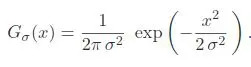
\includegraphics[width=0.5\textwidth]{pics/Gaussian-Filter-Formula-2.jpeg}
    \caption{Gauß-Kernel}
    \cite{GBfilteredPicture2}
    \label{fig:anpr_3}
    \end{figure}
    G\(\sigma\) ist ein räumlicher Gauß, der den Einfluss der entfernten Pixel verringert. Der Abstand zwischen den Pixeln wird mit \(G\sigma(\|p-q\|)\) angegeben. Hierbei ist \(\sigma\) die Ausdehnung der Nachbarschaft.\\
    Der Gaußsche-Unschärfefilter untersucht nur naheliegende Pixel bei der Filterung. Es wird nicht berücksichtig, ob die Pixel die selbe Intensität haben, oder ob die Pixel am Rand liegen oder nicht. Daher werden auch Kanten verwischt, was zu einem Verlust wichtiger Details führt. Die bilaterale Filterung verwendet ebenfalls einen Gauß-Filter im Raum, berücksichtigt aber zusätzlich einen weiteren Gauß-Filter welcher eine Funktion der Pixeldifferenz ist. Die Gaußsche Funktion des Raums sorgt dafür, dass nur nahe gelegene Pixel für die Unschärfe berücksichtigt werden, während die Gaußsche Funktion der Intensitätsdifferenz dafür sorgt, dass nur die Pixel mit ähnlichen Intensitäten wie das zentrale Pixel für die Unschärfe berücksichtigt werden. So bleiben die Kanten erhalten, da die Pixel an den Kanten große Intensitätsunterschiede aufweisen.
    Der wichtige Punkt, der bei der bilateralen Filterung berücksichtigt wird, ist, dass zwei Pixel nicht nur dann nahe beieinander liegen, wenn sie dies räumlich tun, sondern auch, wenn sie eine gewisse Ähnlichkeit im photometrischen Bereich aufweisen. Diese Eigenschaften der bilateralen Filterung überwinden den Nachteil anderer Techniken wie \textit{Averaging Blur} oder \textit{Gaussian Blur}, da sie in der Lage ist, Kanten zu erhalten.\\
    Der Bilaterale Filter wird wie folgt berechnet:
    \begin{figure}[H]
        \centering
        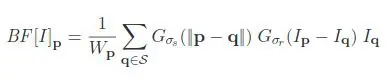
\includegraphics[width=0.5\textwidth]{pics/Bilateral-Filtering-in-Python-OpenCV.jpeg}
        \caption{Bilaterale Filterung Formel}
        \cite{BilateralFormula1}
        \label{fig:anpr:bilat:1}
        \end{figure}
W ist ein Normalisierungsfaktor, welcher mit folgender Formel berechnet wird:
\begin{figure}[H]
    \centering
    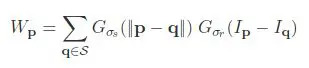
\includegraphics[width=0.5\textwidth]{pics/Bilateral-Filtering-in-Python-OpenCV-Formula2.jpeg}
    \caption{Formel des Normalisierungsfaktors Wp}
    \cite{BilateralFormula2}
    \label{fig:anpr:bilat:2}
    \end{figure}
Dem Gaußschen Filter werden 2 neue Terme hinzugefügt, um den bilateralen Filter zu erhalten. Diese Terme sind:
 \begin{figure}[H]
    \centering
    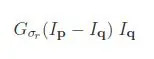
\includegraphics[width=0.3\textwidth]{pics/Bilateral-Filtering-in-Python-OpenCV-Formula3.jpeg}
    \caption{Term 1}
    \cite{BilateralFormula3}
    \label{fig:anpr:bilat:3}
    \end{figure}
\begin{figure}[H]
        \centering
        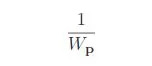
\includegraphics[width=0.3\textwidth]{pics/Bilateral-Filtering-in-Python-OpenCV-Formula4.jpeg}
        \caption{Term 2}
        \cite{BilateralFormula4}
        \label{fig:anpr:bilat:4}
        \end{figure}
Wie aus der Gauß-Filterung bereits bekannt, ist\textit{G\(\sigma\)s} ein räumlicher Gauß, welcher den Einfluss enfernter Pixel verringert. Der zweite Term ist \textit{G\(\sigma\)r}, ein Bereichs-Gauß, welcher Einflüsse von Pixeln \textit{q} mit anderen Intensitätswerten als \textit{Ip} verringert. Bereich bedeutet n diesem Fall Größen, die sich auf Intensitäten beziehen, wohingegen der Raum die Lage der Pixel beschreibt.\\
\textit{\(\sigma\)s} ist ein Raumparameter, der für die räumliche Ausdehnung der Kernelgröße in der betrachteten Nachbarschaft beschreibt, und \textit{\(\sigma\)r} hingegen ein Entfernungsparameter, welcher die minimale Amplitude einer Kante beschreibt. Zusammen ergeben die Parameter das Ausmaß der Filterung des Bildes \textit{I}.\\
Daraus folgt:
\begin{compactenum}
    \item Jedes Pixel erhält einen Durchschnitt der benachbarten Pixel, mit dem es überschrieben wird.
    \item Jedes benachbarte Pixel wird durch eine räumliche Komponente, die entfernte Pixel bestraft, und eine Bereichskomponente, die Pixel mit unterschiedlicher Intensität bestraft, gewichtet.
    \item Die Kombination der beiden Komponenten stellen sicher, dass nur nahe, ähnliche Pixel zur Berechnung des Ergebnisses berücksichtigt werden.
\end{compactenum}
Die beiden Parameter \textit{\(\sigma\)r} und \textit{\(\sigma\)s} beeinflussen den bilateralen Filter, indem bei Erhöhung des Entfernungsparameter \textit{\(\sigma\)r} das Ergebnis dem einer Gaußschen Unschärfe ähnelt, und die Erhöhung des räumlichen Parameters \textit{\(\sigma\)s} zur Glättung von großen Merkmalen führt. Veranschaulicht kann dies durch folgende Grafik werden:
\begin{figure}[H]
    \centering
    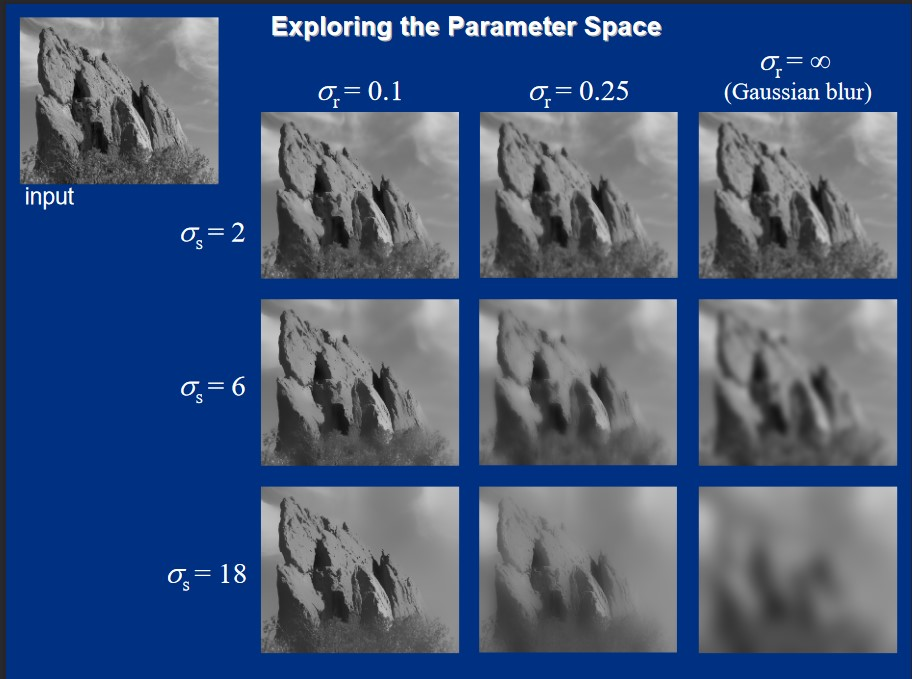
\includegraphics[width=0.5\textwidth]{pics/ParameterBeeinflussungBilateralFilter.jpg}
    \caption{Beeinflussung durch Veränderung der Parameter \textit{\(\sigma\)s} und \textit{\(\sigma\)r}}
    \cite{ParameterBilat}
    \label{fig:anpr:bilat:parameter}
    \end{figure}


Bei der Verwendung der Funktion \verb|cv2.bilateralFilter()| sind folgende Parameter zu berücksichtigen:
\begin{itemize}
    \item \textit{src: } Ein Bild, auf das die Filterung angewendet wird.
    \item \textit{dst: } Das Ergebnis der Filterung. Das Zielbild hat die selbe Größe und den selben Datentyp wie das Ausgangsbild \verb|src|.
    \item \textit{d: }Durchmesser der Pixel-Nachbarschaften, welche zur Berechnung des Filters verwendet werden. Wird dieser negativ, kann auf eine Berechnung durch \textit{sigmaSpace} zurückgegriffen werden.
    \item \textit{sigmaColor: } Ein größerer Wert des Parameters bedeutet, dass weiter entfernte Farben innerhalb der Pixelnachbarschaft zusammengemischt werden, was zu größeren Bereichen mit annähernd gleicher Farbe führt.
    \item \textit{sigmaSpace: }Ein größerer Wert des Parameters bedeutet, dass weiter entfernte Pixel sich gegenseitig beeinflussen, solange ihre Farben nahe genug beieinander liegen. Wenn \textit{d>0} ist, gibt er die Größe der Nachbarschaft unabhängig von sigmaSpace an. Andernfalls ist d proportional zu sigmaSpace.
    \item \textit{borderType: }Randmodus, der für die Extrapolation von Pixeln außerhalb des Bildes verwendet wird.
\end{itemize}
\cite{Filter}
\subsubsection{Kantenerkennung \label{sec:anpr:kantenerkennung}}
Die Kantenerkennung wird mit dem Aufruf von \verb|cv2.Canny()| durchgeführt. Diese Funktion wurde von John F. Canny entwickelt, und ist ein mehrstufiger Algorithmus, welcher in 4 Stufen aufgeteilt werden kann:
\begin{compactenum}
    \item \textit{Rauschunterdrückung: }
    \begin{compactenum}
        \item Da die Kantenerkennung anfällig für Bildrauschen ist, wird zunächst das Bildrauschen mit einem 5x5-Gauß-Filter entfernt
    \end{compactenum}
    \item \textit{Ermittlung des Intensitätsgradienten des Bildes: }
    \begin{compactenum}
        \item  Das geglättete Bild wird dann mit einem Sobel-Kernel sowohl in horizontaler als auch in vertikaler Richtung gefiltert, um die erste Ableitung in horizontaler Richtung \((Gx)\) und vertikaler Richtung \((Gy)\) zu erhalten. Aus diesen beiden Bildern können der Kantengradienten und die Richtung für jedes Pixel wie folgt ermittelt:
        \begin{equation}
            \begin{split}
                \begin{aligned}
                    \text{Kantengradient (G)} &= \sqrt{G^2x+G^2y}\\
                    \text{Winkel (\(\theta\))} &= \tan^{-1}(\frac{Gy}{Gx})
                \end{aligned}
            \end{split}
        \end{equation}
        \item Die Richtung der Steigung ist immer senkrecht zu den Kanten. Sie wird auf einen von vier Winkeln gerundet, welche die vertikale, horizontale und zwei diagonale Richtungen darstellen.
    \end{compactenum}
    \item \textit{Non-Maximum-Suppression: }
    \begin{compactenum}
        \item Nachdem Gradient und Richtung ermittelt wurden, wird das Bild vollständig gescannt, um alle unerwünschten Pixel zu entfernen, die möglicherweise nicht die Kante bilden. Zu diesem Zweck wird bei jedem Pixel geprüft, ob es in dessen Umgebung ein lokales Maximum in der Richtung des Gradienten darstellt.
        \begin{figure}[H]
            \centering
            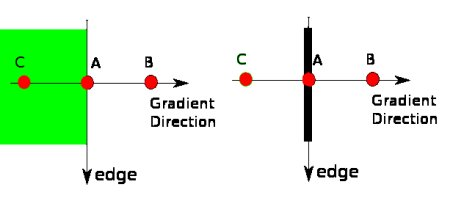
\includegraphics[width=0.5\textwidth]{pics/nms.jpg}
            \caption{Non-Maximum-Suppression}
            \cite{NMSPic}
            \label{fig:anpr:edge:nms}
            \end{figure}
            Punkt A befindet sich auf der Kante in vertikaler Richtung. Die Richtung des Gradienten ist normal zur Kante. Die Punkte B und C liegen in Gradientenrichtung. Punkt A wird also mit den Punkten B und C daraufhin überprüft, ob er ein lokales Maximum bildet. Wenn ja, wird er für die nächste Stufe berücksichtigt, andernfalls wird er unterdrückt (auf Null gesetzt).Das Ergebnis ist ein Binärbild mit dünnen Rändern.
    \end{compactenum}
    \item \textit{Hysterese-Schwellenwertbildung: }
    \begin{compactenum}
        \item  In dieser Phase wird entschieden, welche Kanten wirklich Kanten sind und welche nicht. Hierfür werden zwei Schwellenwerte benötigt, minVal und maxVal. Alle Kanten, deren Intensitätsgradient größer als maxVal ist, sind sicher, dass es sich um Kanten handelt, und diejenigen, die unter minVal liegen, sind sicher, dass es sich um Nicht-Kanten handelt, und werden daher verworfen. Diejenigen, die zwischen diesen beiden Schwellenwerten liegen, werden auf der Grundlage ihrer Konnektivität als Kanten oder Nicht-Kanten klassifiziert. Wenn sie mit "\textit{sure-edge}"-Pixeln verbunden sind, werden sie als Teil von Kanten betrachtet. Andernfalls werden sie ebenfalls verworfen.
        \begin{figure}[H]
            \centering
            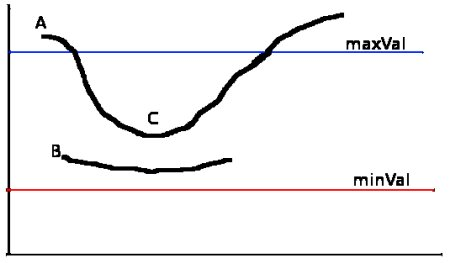
\includegraphics[width=0.5\textwidth]{pics/hysteresis.jpg}
            \caption{Hysterese-Schwellenwertbildung}
            \cite{hysteresisPic}
            \label{fig:anpr:edge:hysteresis}
            \end{figure}
            Die Kante A liegt oberhalb von maxVal, wird also als \"sichere Kante\" betrachtet. Obwohl die Kante C unter maxVal liegt, ist sie mit der Kante A verbunden, so dass sie ebenfalls als gültige Kante betrachtet wird und in der vollständigen Kurve enthalten ist. Aber die Kante B, obwohl sie oberhalb von minVal liegt und in der gleichen Region wie die Kante C ist, ist nicht mit einer \"sicheren Kante\" verbunden, so dass sie verworfen wird. Es ist also sehr wichtig, dass minVal und maxVal entsprechend ausgewählt werden, um das richtige Ergebnis zu erhalten.
            In dieser Phase werden auch kleine Pixel entfernt, wobei davon ausgegangen wird, dass die Kanten lange Linien sind. Dadurch enstehen starke Kanten im Bild.
    \end{compactenum}
\end{compactenum}
Angewendet auf ein Graustufenbild, sieht das Ergebnis der Kantenerkennung wie folgt aus:
\begin{figure}[H]
    \centering
    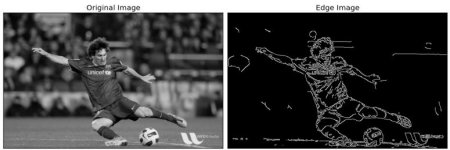
\includegraphics[width=0.8\textwidth]{pics/canny1.jpg}
    \caption{Ergebnis der Kantenerkennung}
    \cite{CannyPic}
    \label{fig:anpr:edge:canny}
    \end{figure}
\subsubsection{Konturenfindung}
Konturen können einfach als eine Kurve erklärt werden, die alle kontinuierlichen Punkte (entlang der Grenze) verbindet, die dieselbe Farbe oder Intensität haben. Die Konturen sind ein nützliches Werkzeug für die Formanalyse und die Erkennung von Objekten.
Mit dem Ergebnis der Kantenerkennung aus \ref{sec:anpr:kantenerkennung} kann OpenCV Konturen eines weißen Objekts vor einem schwarzen Hintergrund finden. Dies geschieht mit dem Aufruf von \verb|cv2.findContours(thresh, cv.RETR_TREE, cv.CHAIN_APPROX_SIMPLE)|. Die Parameter können wie folgt beschrieben werden:
\begin{compactenum}
    \item \textit{thresh}: Das Bild, auf das die Konturen gesucht werden sollen.
    \item \textit{mode}: Der Modus, der zur Konturensuche verwendet wird.
    \item \textit{method}: Die Methode, die zur Konturennäherung verwendet wird.
\end{compactenum}
Als Rückgabewert gibt die Funktion die Konturen und die Hierarchie aus. Die Konturen sind eine Python-Liste mit allen Konturen im Bild. Jede einzelne Kontur ist ein Numpy-Array mit (x,y)-Koordinaten von Grenzpunkten des Objekts.
Der dritte Parameter, die Konturennäherungsmethode, bestimmt, welche Begrenzungspunkte gespeichert werden. Bei \verb|cv2.CHAIN_APPROX_NONE| werden alle Punkte der Kontur gespeichert. Dies ist aber nicht nötig, da nur der Start- und Endpunkt der Linie benötigt werden. Daher ist es sinnvoller, \verb|cv2.CHAIN_APPROX_SIMPLE| zu verwenden, da diese Methode alle überflüssigen Punkte entfernt und die Konturen komprimiert, um so Speicherplatz zu sparen.
In Abbildung \ref{fig:anpr:contour:cam} wird der Unterschied der beiden Methoden erkenntlich gemacht. Anstelle von 734 Punkten bei der Verwendung von \verb|cv2.CHAIN_APPROX_NONE| werden bei \verb|cv2.CHAIN_APPROX_SIMPLE| nur die Start- und Endpunkte der Konturen und damit insgesamt 4 Punkte gespeichert.\cite{drawContours}
\begin{figure}[H]
    \centering
    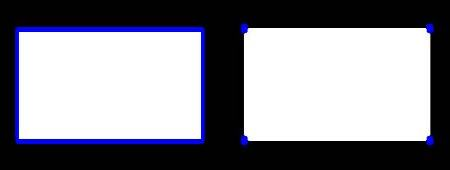
\includegraphics[width=0.8\textwidth]{pics/none.jpg}
    \caption{Unterschied von}
    \cite{CAMPic}
    \label{fig:anpr:contour:cam}
    \end{figure}
\subsubsection{Überprüfung der Konturen}
Im nächsten Schritt wird mittels \verb|imutils.grab_contours| überprüft, welche OpenCV Version verwendet wird. Dies unterscheidet sich in der Länge des Kontur-Tupels:
\begin{itemize}
    \item Ist das Tupel 2 Elemente lang, handelt es sich um OpenCV v2.4, v4-beta oder v4-official
    \item Ist das Tupel 3 Elemente lang, handelt es sich um OpenCV v3, v4-pre oder v4-alpha
\end{itemize}
\cite{imutilsGrabContours}\\
Nachdem die Konturen sortiert wurden, wird der Konturumfang mit \verb|cv2.arcLength| berechnet. Danach wird die Kontur unter Verwendung des Douglas-Peucker-Algorithmus mit dem vorher berechneten Konturumfang angepasst. Kommt dieser zu keinem Ergebnis, wird die Kontur verworfen und eine Fehlermeldung ausgegeben.\\
Wurde jedoch eine geschlossene Kontur mit 4 Eckpunkten gefunden, beginnt die Funktion \verb|cv2.drawContours| mit der Zeichnung der Kontur. Die Funktionsparameter sind zum Einen das Bild, auf das die Kontur gezeichnet werden soll, und zum anderen die Kontur. Weitere Parameter, wie Farbe, Dicke und mehr können ebenfalls übergeben werden.
\cite{drawContours}
\subsubsection{Maskieren der relevanten Bildregion \label{sec:anpr:mask}}
Da für den weiteren Ablauf des Programms nur noch die Region, in der sich das Kennzeichen befindet, relevant ist, wird diese maskiert und als neues Bild gespeichert: 

\begin{lstlisting}[language=Python, caption=Maskieren der Kennzeichenregion und Abspeichern in neuem Bild, label=lst:impl:anpr:mask]
    mask = np.zeros(gray.shape, np.uint8)
    new_image = cv2.drawContours(mask, [screenCnt], 0, 255, -1,)
    new_image = cv2.bitwise_and(frame, frame, mask=mask)
    (x, y) = np.where(mask == 255)
    (topx, topy) = (np.min(x), np.min(y))
    (bottomx, bottomy) = (np.max(x), np.max(y))
    Cropped = gray[topx:bottomx+1, topy:bottomy+1]
\end{lstlisting}

\subsubsection{Texterkennung \label{sec:anpr:text}}
Aus dem in \ref{sec:anpr:mask} erzeugten Bild kann nun der Text des Kennzeichens gelesen werden. Dies geschieht mit der Funktion : 
\begin{lstlisting}[language=Python, caption=Maskieren der Kennzeichenregion und Abspeicher in neuem Bild, label=lst:impl:anpr:text]
    text = pytesseract.image_to_string(Cropped, config='--psm 11')
\end{lstlisting}

Mit \verb|config='--psm 11'| wird die Priorität der Texterkennung auf den Text selbst gesetzt. Da zuvor schon alle irrelevanten Bereiche des Bildes durch Maskieren entfernt wurden, wurde hier diese Priorität verwendet, um die Ergebnisse der Kennzeichenerkennung zu verbessern. \cite{PSM11} \\
Dadurch kann es aber auch zu Problemen kommen, da nun Sonderzeichen erkannt werden, welche nicht auf dem Kennzeichen existieren. Um alle Leerzeichen und Sonderzeichen zu entfernen, wurden mit \verb|re.sub('[^a-zA-Z0-9 \n\.]', '', text)| alle nicht möglichen Zeichen aus dem Text entfernt.


\subsubsection{Überprufung des erkannten Kennzeichens}
Der Text aus \ref{sec:anpr:text} wird mit dem Aufruf des Modules \verb|checkPlate(text_replaced)| an ein Python-Script übergeben, welches für die weitere Überprüfung zuständig ist. 

\begin{lstlisting}[language=Python, caption=Abfrage der Kennzeichen aus der Datenbank, label=lst:impl:anpr:check:db]
    print(type(text))
    r = requests.get('http://130.162.215.116/get-licenseplates')
    val = json.loads(r.text)
\end{lstlisting}

Im Code-Abschnitt \ref{lst:impl:anpr:check} wird die Antwort des Servers in ein JSON-Objekt geladen und mit \verb|json.loads| in ein Python-Objekt umgewandelt, welches die Daten der gefundenen Kennzeichen enthält. Da die Formatierung der Kennzeichen aus der Datenbank sich von dem der Ergebnis der Erkennung unterscheiden kann, wird mit \verb|str.maketrans| eine Zuordnungstabelle erstellt, die im späteren Verlauf von der Methode \verb|str.translate| verwendet wird, um die Formatierungsunterschiede zu beseitigen.\\
Kennzeichen können im Dashboard deaktiviert werden und dürfen in diesem Zustand nicht die Garage öffnen. Um dies zu realisieren, wird der Boolean \verb|active| aus der Datenbankabfrage jedes Kennzeichens überprüft. Wenn dieser Boolean auf \verb|False| steht, wird das Kennzeichen nicht weiter überprüft. 

 \begin{lstlisting}[language=Python, caption=Überprüfung auf Gleichheit der beiden Strings, label=lst:impl:anpr:check]
    if text.replace(" ", "").translate(table) == value["licenseplate"].translate(table).replace(" ", ""):
        print("licenseplate recognized, initiating opening sequence")
        initiateOpeningSequence()
    else:
        print("not recognized, staying closed")
 \end{lstlisting}
 Sind beide Kennzeichen gleich, wird die Methode \verb|initiateOpeningSequence| aufgerufen, welche das Relais ansteuert.